%%%%%%%%%%%%%%%%%%%% author.tex %%%%%%%%%%%%%%%%%%%%%%%%%%%%%%%%%%%
%
% sample root file for your "contribution" to a proceedings volume
%
% Use this file as a template for your own input.
%
%%%%%%%%%%%%%%%% Springer %%%%%%%%%%%%%%%%%%%%%%%%%%%%%%%%%%


\documentclass{svproc}
%
% RECOMMENDED %%%%%%%%%%%%%%%%%%%%%%%%%%%%%%%%%%%%%%%%%%%%%%%%%%%
%

% to typeset URLs, URIs, and DOIs
\usepackage{url}
\usepackage{amsmath}
\usepackage{algorithm}
\usepackage[noend]{algpseudocode}

\usepackage{graphicx}

\usepackage{caption}
\usepackage{subcaption}


\captionsetup{compatibility=false}

\usepackage{amsmath}
\usepackage{tikz}
\usepackage{adjustbox}

\usetikzlibrary{arrows, arrows.meta, fit, positioning, quotes,
                shadows, shapes.geometric, shapes.misc}





\def\UrlFont{\rmfamily}

%%%%%%%%%%%%% math stuff
\usepackage{amssymb}

%flowchart definitions
\tikzstyle{startstop} = [rectangle, rounded corners, minimum width=3cm, minimum height=1cm,text centered, draw=black, fill=red!30]
\tikzstyle{io} = [trapezium, trapezium left angle=70, trapezium right angle=110, minimum width=3cm, minimum height=1cm, text centered, draw=black, fill=blue!30]
\tikzstyle{process} = [rectangle, minimum width=1cm, minimum height=1cm, text centered, draw=black, fill=orange!30]
\tikzstyle{decision} = [diamond, minimum width=1cm, minimum height=1cm, text centered, draw=black, fill=green!30]
\tikzstyle{arrow} = [thick,->,>=stealth]

\tikzset{
  font={\fontsize{11pt}{12}\selectfont}}


% vectors in bold
\newcommand{\vp}{\mathbf{p}}
\newcommand{\valpha}{\mathbf{\alpha}}
\newcommand{\vP}{\mathbf{P}}
\newcommand{\vg}{\mathbf{g}}
\newcommand{\vf}{\mathbf{f}}
\newcommand{\vw}{\mathbf{w}}
\newcommand{\vx}{\mathbf{x}}
\newcommand{\vq}{\mathbf{q}}
\newcommand{\vzero}{\mathbf{0}}
\newcommand{\vn}{\mathbf{n}}
\newcommand{\vo}{\mathbf{o}}


% sets as caligraphics
\newcommand{\cV}{\mathcal{V}}
\newcommand{\cS}{\mathcal{S}}

% misc
\newcommand{\R}{\mathbb{R}} % real numbers

%%%%%%%%%%%%%

\begin{document}
\mainmatter              % start of a contribution
%
% Robust Motion Execution
% 
\title{Distributed Realtime Trajectory Replanning for Robust Motion Execution in Multi-Robot Systems}


%
\titlerunning{Distributed Realtime Trajectory Replanning}  % abbreviated title (for running head)
%                                     also used for the TOC unless
%                                     \toctitle is used
%
\author{Baskin Senbaslar \and Wolfgang H\"onig \and
Nora Ayanian}
%
%\authorrunning{Ivar Ekeland et al.} % abbreviated author list (for running head)
%
%%%% list of authors for the TOC (use if author list has to be modified)
\tocauthor{Baskin Senbaslar, Wolfgang H\"onig, Nora Ayanian}
%
\institute{University of Southern California, Los Angeles CA, USA,\\
\email{\{baskin.senbaslar, whoenig, ayanian\}@usc.edu}}

\maketitle              % typeset the title of the contribution

\begin{abstract}
\keywords{trajectory planning, collision avoidance, multi-robot systems}
\end{abstract}


\section{Introduction}
Motion planning for multi-robot systems is widely used and in particular important in cases where many robots have to interact with each other in confined spaces, potentially with many obstacles around.
Examples include coordination of robots in warehouses~\cite{Kiva}, traffic management at intersections~\cite{IntersectionManagementDresner}, and airport management~\cite{AirportTug}.
Modern planning algorithms can find trajectories that effectively coordinate hundreds of robots while approximately optimizing objectives like total energy used~\cite{crazyplanning-ieeetro}.
However, all such solutions assume that the resulting trajectories can be executed approximately perfectly, which is in particular not true for teams of hundreds of robots that have to operate persistently.

We propose robust motion execution as a framework that can take pre-planned trajectories as input and compensate for a variety of dynamic changes, including imperfect motion execution of some robots, newly appearing obstacles, or robots breaking down.
Our framework is fully distributed and requires no communication; the robots only need to know their own trajectories and need to be able to sense their neighbors' positions and obstacles around them.

Robust motion execution is an extension of cooperative collision avoidance where our objective is to stay close to the originally planned trajectories as much as possible.
In contrast, traditional collision avoidance methods frequently only take a desired velocity, desired goal state, or desired action as input (see Section~\ref{sec:relatedWork}).
Our method is based on \emph{Buffered Voronoi Cells} (BVC)~\cite{bufferedVoronoiCells} as the underlying cooperative collision avoidance strategy and retains the same theoretical guarantees.
At the high-level we employ a novel combination of trajectory optimization and discrete search-based planning.
The discrete search allows us to avoid local minima effectively even in difficult scenarios, while the trajectory optimization takes the dynamics of real physical robots into account.\footnote{test footnote}

% todo: perhaps write some more about what experiments we did, after we have the material

\section{Problem Formulation}
% assumptions: circular robots; robots follow the same rules; static (or slow) obstacles
% input: original curves; positions of peers; dynamic limits; environment (at least able to sense); dt; curve_count; T
% output: at each dt: new trajectory such that there is no collision (guaranteed)
% issues: no live-lock guarantee
We solve our problem completely in a distributed fashion. No central authority coordinates the robots and robots themselves can't communicate with their peers, hence they have no information about the plans of other robots. In every time step $K$, seperated by replanning period $\delta t$, each robot $i$ solves the following problem:
\begin{align*}
    \text{Given,}\ \ \ \ \ &\\
    \vo^i(t')&:\text{ original trajectory of robot $i$},\\
    ct&:\text{ current global time},\\
    \delta t&:\text{ replanning period},\\
    \tau&: \text{time horizon},\\ 
    c&:\text{ maximum continuity between pieces},\\
    \Theta&:\text{ occupancy grid of the environment},\\
    \{\vp_i\}&:\text{ set of positions of all robots},\\
    \gamma&: \text{ dynamic limits of robots in any derivation degree},\\
    &\ \ \ \ \gamma_j \text{ being the limit for $j^{th}$ derivation degree}\\
    \text{find a new}&\text{ trajectory $\vf_K^i(t)$ such that},\\
    \vf_K^i(t)&\text{ is}\text{ continuous up to degree $c$ for }t\in [0,\tau],\\
    \frac{d^j\vf_K^i(t)}{dt^j}(0) &= \frac{d^j\vf_{K-1}^i(t)}{dt^j}(\delta t)\text{ for } j\in\{0,1,...,c\}\\
    \vf_K^i(t)&\text{ is collision free for $t\in [0,\delta t]$},\\
    \vf_K^i(t)&\text{ tracks $\vo^i(t')$ as close as possible for $t\in[0,\tau]$ or equivalently $t'\in[ct, ct+\tau]$ }, \text{and}\\
    \left\|\frac{d^j \vf^i(t)}{dt^j}\right\| &\leq \gamma_j\text{ for } t\in [0,\tau],\\
\end{align*}

Robot $i$'s trajectory $f^i(t)$ is $f_K^i(t)$ in $K^{th}$ time step. It follows the trajectory for $\delta t$ seconds, and replans to calculate $f_{K+1}^i(t)$ and replaces $f^i(t)$ with it.

\section{Preliminaries}

\subsection{Buffered Voronoi Cells}
Given a set of $m$ robots with positions $\vp_1,\vp_2,\ldots,\vp_m \in \R^n$ and radii $r_1,r_2,...r_m \in \R$, the buffered voronoi cell $\cV_i$ of robot $i$ is defined as~\cite{bufferedVoronoiCells}:
\begin{align}
    \cV_i &= \left\{\vp : \forall_{j\neq i} \frac{\vp_j-\vp_i}{\|\vp_j-\vp_i\|}\cdot \vp - \frac{\vp_j-\vp_i}{\|\vp_j-\vp_i\|}\cdot \frac{\vp_j+\vp_i}{2} + r_i\leq 0 \right\} \label{voronoi_cell_definition}
\end{align}
where $\|\vp\|$ is the L2-norm of vector $\vp$.

The inequality inside \eqref{voronoi_cell_definition} defines a hyperspace $\cS_i^j$ that is bounded by hyperplane $H_i^j$ that separates point $\vp_i$ from $\vp_j$ with normal $\valpha_i^j$ and distance along normal $\beta_i^j$ where $\valpha_i^j\in \R^n$ and $\beta_i^j\in \R$ such that
\begin{align*}
    \valpha_i^j &= \frac{\vp_j - \vp_i}{\|\vp_j-\vp_i\|}\\
    \beta_i^j &= \valpha_i^j \cdot \left(\frac{\vp_i + \vp_j}{2}\right) - r_i.
\end{align*}

The set of all buffered voronoi cells is called the buffered voronoi decomposition of the space. For a given buffered voronoi decomposition of the space, any point $\vp\in \R^n$ can be inside one of the buffered voronoi cells at most. We are using this fact in order to guarantee robot-to-robot collision avoidance.

The hyperspace $\cS_i^j$ has the following definition:
\begin{align}
    \cS_i^j = \left\{\vp : \valpha_i^j \cdot \vp - \beta_i^j \leq 0\right\}
\end{align}
Using this definition, an equivalent definition for the set \eqref{voronoi_cell_definition} is
\begin{align}
    \cV_i = \bigcap\limits_{j\neq i} \cS_i^j. \label{voronoi_intersection_definition}
\end{align}
This definition suggests a natural algorithm to compute the buffered voronoi cell of any robot $i$ in terms of the hyperplanes $H_i^j$:
\begin{algorithmic}[1]
    \Function{Voronoi}{[$p_i$]: robot positions, $i$: robot that we want to calculate voronoi cell of, $r_i$: radius of robot $i$}
        \State $H = \{\}$
        \ForAll{$j\neq i$}
            \State $H_i^j = (\alpha_i^j, \beta_i^j)$
            \State $H = H\cup H_i^j$
        \EndFor
        \State \Return $H$
    \EndFunction
\end{algorithmic}
This is an $O(m)$ operation, $m$ being the number of robots.


\subsection{B\'ezier Curves}
A degree $d$ b\'ezier curve $\vg(t)$ parametrized by duration $T$ is defined by $d+1$ control points $\vP_0, \vP_1, ..., \vP_d \in \R^n$ such that
\begin{align}
    \vg(t; T) = \sum_{i=0}^d \vP_i {d\choose i}\left(\frac{t}{T}\right)^i\left(1-\frac{t}{T}\right)^{d-i},\hskip .5cm 0\leq t \leq T
\end{align}

The curve starts at $\vP_0$ and ends at $\vP_d$. It does not interpolate the control points, but uses them to guide the curve. A b\'ezier curve lies completely inside the convex hull of its control points \cite{Bernstein}. We use this property to give robot-to-robot and robot-to-obstacle no-collision guarantees.

We use polynomial splines as trajectories where each piece is a b\'ezier curve. Given a trajectory $\vf^i(t)$ for robot $i$ with $l$ pieces, $T^i_j$ denotes the duration of $j^{th}$ piece, $\vf^i_j(t; T^i_j)$ denotes the $j^{th}$ piece of the trajectory, $\vP^i_{j,k}$ denotes the $k^{th}$ control point of $j^{th}$ piece, and $P^i_{j,k,u}$ denotes the $u^{th}$ coordinate of that control point where $j \in \{1,2,...,l\}$, $k \in \{0,1,...,d\}$, $u \in \{1,2,...,n\}$.


\subsection{Support Vector Machine}
Support vector machine is a supervised learning method that is used to classify data into several classes. In binary classification problems, given linearly separable data set $\{(\vx_i, y_i)\}$ where $\vx_i \in \R^n$ is a data point and $y_i \in \{-1, 1\}$ is the corresponding class label, SVM problem tries to find a hyperplane with normal $\vw$ and distance along the normal $b$ that separates two classes. SVM problem for binary classification with separable data set can be stated as the following quadratic optimization problem with hard constraints \cite{SVM}:
\begin{align*}
    \text{minimize}\ \ \  &\|\vw\|\\
    \text{subject to}\ \ \  & y_i(\vw \cdot \vx_i - b) \geq 1
\end{align*}
We use SVMs to define collision free convex subspaces that are obstacle-free.
\subsection{Trajectory Optimization}
We present our replanning problem as a quadratic optimization problem where the control points of the trajectory are the variables. The overall structure of quadratic optimization problems is as follows \cite{qpOASES}:
\begin{align*}
    \text{minimize}\ \ \ &\frac{1}{2}\vx^TH\vx + \vx^Tg\\
    \text{subject to}\ \ \ & lbA \leq A\vx \leq ubA\\
    &lb \leq \vx \leq ub
\end{align*}

Each constraint on the problem appends a set of rows to the matrices $A$, $lbA$, and $ubA$. There are 4 types of constraints we impose: starting point constraints, end point constraints, continuity constraints and hyperplane constraints.
\subsubsection{Initial Point Constraints}
For each of the curves in the trajectory, we can impose initial point constraints. An initial point constraint requires curve to have a specific value in any order of its derivatives in the beginning. $S_j(D, T)$ is the matrix we append to $A$ in order to evaluate curve $j$ at its starting point, $D$ being the degree of derivation, $T$ being the duration of the curve.

The value of the curve in the beginning is simply a linear combination of the control points. The rows of $S_j$ are the coefficients of control points in this linear combination, each of which corresponding to a different dimension. We append the desired vector $\vq$ for the constraint to both $lbA$ and $ubA$ matrices. Note that by adding the same vector to both upper and lower bound matrices, we impose an equality constraint.
\subsubsection{End Point Constraints}
This is essentially same with starting point constraints. Only difference is that instead of evaluating the curve at $t=0$, we evaluate it at $t=T$.

$E_j(D,T)$ denotes the matrix we append to $A$ in order to evaluate the curve $j$ at its end point, $D$ being the degree of derivation, $T$ being the duration of the curve. We again append desired value vector $\vq$ to both $lbA$ and $ubA$.
\subsubsection{Continuity Constraints}
For each consecutive curves $j$ and $j+1$ in the trajectory, we can impose a continuity constraint of any degree $D$. We basically take the difference of the $D^{th}$ derivative of curve $j$ evaluated at time $t=T_j$ and the $D^{th}$ derivative of curve $j+1$ evaluated at time $t=0$ and require it to be $\vzero$. This difference is again a linear combination of the control points.

$C_j(D,T_j,T_{j+1})$ denotes the matrix we append to A in order to calculate the difference between curves $j$ and $j+1$, $D$ being the degree of derivation, $T_j$ being the duration of curve $j$ and $T_{j+1}$ being the duration of curve $j+1$. We append $\vzero$ to both $lbA$ and $ubA$.
\subsubsection{Hyperspace Constraints}
For each of the control points, we can add a hyperplane constraint that requires the point not to be in the positive side of the hyperplane. Given hyperplane with normal $\vn$ and distance along the normal $d$, not-positive side of the hyperplane is simply the set $J$ defined as
\begin{align*}
    J = \left\{\vp: \vn \cdot \vp - d \leq 0\right\}
\end{align*}

The constraint is again a linear combination of control points. $H_{j,k}(\vn)$ denotes the row we append to $A$ in order to impose a hyperplane constraint on the $k^{th}$ control point of $j^{th}$ curve, $\vn$ being the normal of the hyperplane. We add $d$ to $ubA$ and $-\infty$ to $lbA$.
\\

Notice that $S_j, E_j, C_j$ and $H_{j,k}$ matrices defined above also depend on the problem dimension $n$ and number of control points per curve $d+1$. To not to complicate the notation, we omitted these details in the symbols. In our treatment, we do not change the number of control points per curve and the dimension of the problem between replanning iterations. Therefore, omitting these details does not present any problems in terms of the completeness of our explanation. In any instance, dimension and points per curve will be inferred from the context.
\section{Approach}

% TODO: running example?

\subsection{Approach Overview}
Our approach has three big components: \emph{discrete planning} that is used in case using only optimization may present problems, \emph{trajectory optimization} to optimize trajectory while avoiding obstacles and other robots, and \emph{dynamic rescaling} to comform to the dynamic limits of the robot.

In each iteration, pipeline that is summarized in figure \ref{fig:flowchart} gets executed. Period of each iteration is $\delta_t$, and all pipeline gets executed every $\delta_t$.

In the beginning of the each iteration, we check for some conditions defined in the following sections to see if we need discrete replanning. If the answer is yes, we do a discrete search that results in a discrete path that is obstacle and robot free. Then, we transform this discrete plan to b\'ezier control points and use those points as the initial data for trajectory optimization. If the answer is no, we skip discrete search, and directly use the control points of the previous plan as the initial data.

Depending on whether we did discrete search or not, we build objective matrix $H$ for trajectory optimization in a slightly different way.

At this point, algorithm has the same flow independent of the fact that we did discrete search or not. We compute $A$ matrix that represents continuity, hyperspace, initial point and end point constraints. Robot-to-robot collision avoidance is enforced with buffered voronoi decomposition of the space while robot-to-obstacle collision avoidance is enforced with SVM hyperspaces that we calculate between trajectory pieces and the obstacles. When the optimization is done, we check whether the dynamic limits are violated. While the answer is yes, we increase durations of pieces and do the optimization again until dynamic limits are not violated. In the end, we have a trajectory $f^i(t)$ that is guaranteed to be collision-free up to time $\delta t$, is $C^{(c)}$ continuous, obeys the dynamic limits of the robot, tries to stay close to the original trajectory and is a good starting point for the next iteration.

\begin{figure}
%\begin{adjustbox}{width=\textwidth,caption={bla}}
\resizebox{\textwidth}{!}{
% \footnotesize
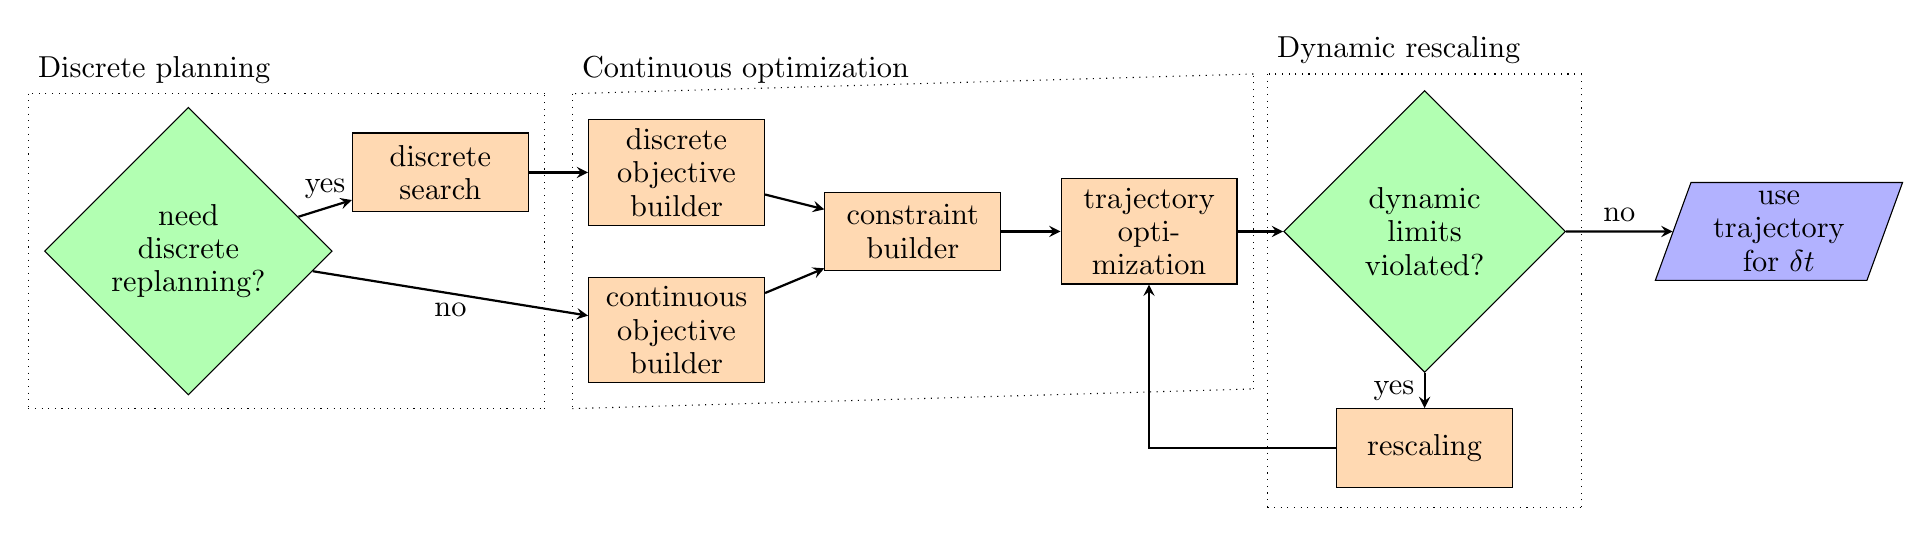
\begin{tikzpicture}[node distance = 2cm]
    \node (discrete) [decision, text width=2cm] {need discrete replanning?};
    \node (discretesearch) [process, right of=discrete, xshift=1.2cm, yshift = 1cm, text width = 2cm] {discrete search};
    \node (discobjbuild) [process, right of=discretesearch, xshift = 1cm, text width = 2cm] {discrete objective builder};
    \node (contobjbuild) [process, below of=discobjbuild, text width = 2cm] {continuous objective builder};
    \node (constraintbuild) [process, right of=discobjbuild, yshift = -0.75cm, xshift = 1cm, text width=2cm]
    {constraint builder};
    \node (trajopt) [process, right of=constraintbuild, xshift = 1cm, text width = 2cm] {trajectory optimization};
    \node (dynamiclimits) [decision, right of=trajopt, xshift = 1.5cm, text width = 2cm] {dynamic limits violated?};
    \node (rescale) [process, below of = dynamiclimits, text width = 2cm, yshift = -0.75cm] {rescaling};
    \node (end) [io, right of = dynamiclimits, text width = 2cm, xshift = 2.5cm] {use trajectory for $\delta t$};
    
    \coordinate[above=2cm of discrete.west, xshift=-0.2cm] (c1);
    \coordinate[below=2cm of discrete.west, xshift=-0.2cm] (c2);
    \coordinate[above=2cm of discretesearch.east, xshift = 0.2cm, yshift=-1cm] (c3);
    \coordinate[below=2cm of discretesearch.east, xshift = 0.2cm, yshift = -1cm] (c4);
    
    
    \coordinate[above=2cm of discobjbuild.west, xshift=-0.2cm, yshift=-1cm] (c5);
    \coordinate[below=2cm of discobjbuild.west, xshift=-0.2cm, yshift = -1cm] (c6);
    \coordinate[above=2cm of trajopt.east, xshift = 0.2cm] (c7);
    \coordinate[below=2cm of trajopt.east, xshift = 0.2cm] (c8);
    
    
    \coordinate[above=2cm of dynamiclimits.west, xshift=-0.2cm, ] (c9);
    \coordinate[below=2cm of dynamiclimits.west, xshift=-0.2cm, yshift = -1.5cm] (c10);
    \coordinate[above=2cm of dynamiclimits.east, xshift = 0.2cm] (c11);
    \coordinate[below=2cm of dynamiclimits.east, xshift = 0.2cm, yshift = -1.5cm] (c12);
    
    \draw [arrow] (discrete) -- node[anchor=south] {yes} (discretesearch);
    \draw [arrow] (discrete) -- node[anchor=north] {no} (contobjbuild);
    \draw [arrow] (discretesearch) -- (discobjbuild);
    \draw [arrow] (discobjbuild) -- (constraintbuild);
    \draw [arrow] (contobjbuild) -- (constraintbuild);
    \draw [arrow] (constraintbuild) -- (trajopt);
    \draw [arrow] (trajopt) -- (dynamiclimits);
    \draw [arrow] (dynamiclimits) -- node[anchor=south] {no} (end);
    \draw [arrow] (dynamiclimits) -- node[anchor=east] {yes} (rescale);
    \draw [arrow] (rescale) -| (trajopt);
    
    \node[right = 0cm of c1, yshift=0.3cm] {Discrete planning};
    \node[right = 0cm of c5, yshift=0.3cm] {Continuous optimization};
    \node[right = 0cm of c9, yshift=0.3cm] {Dynamic rescaling};
    
    \draw [dotted] (c1) -- (c2);
    \draw [dotted] (c2) -- (c4);
    \draw [dotted] (c4) -- (c3);
    \draw [dotted] (c3) -- (c1);
    
    \draw [dotted] (c5) -- (c6);
    \draw [dotted] (c6) -- (c8);
    \draw [dotted] (c8) -- (c7);
    \draw [dotted] (c7) -- (c5);
    
    
    \draw [dotted] (c9) -- (c10);
    \draw [dotted] (c10) -- (c12);
    \draw [dotted] (c12) -- (c11);
    \draw [dotted] (c11) -- (c9);
\end{tikzpicture}
}
%\end{adjustbox}
\caption{Overview of the replanning pipeline.
}
\label{fig:flowchart}
\end{figure}

\begin{figure}
\centering
\begin{subfigure}[t]{0.45\textwidth}
\centering
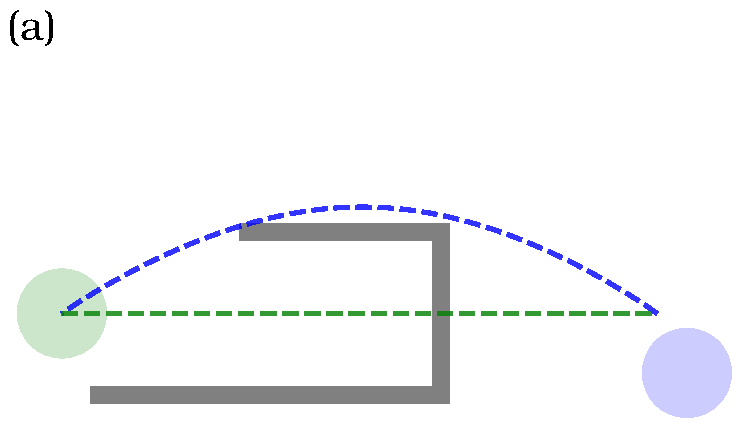
\includegraphics[width=.9\textwidth]{images/swap2_initial.pdf}
\caption{Initial configuration.}
\label{fig:swap2:initial}
\end{subfigure} \hfill
\begin{subfigure}[t]{0.45\textwidth}
\centering
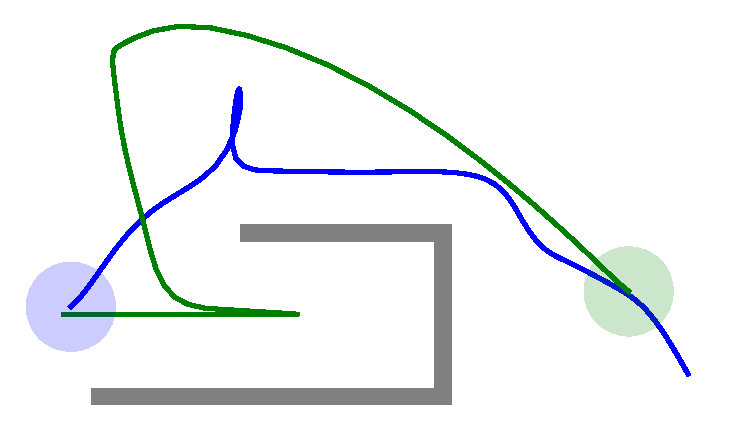
\includegraphics[width=.9\textwidth]{images/swap2_final.pdf}
\caption{Final configuration and executed trajectories.}
\label{fig:swap2:final}
\end{subfigure}
\caption{Two robots (green and blue circles) are tasked with following their preplanned trajectories (green and blue dashed lines).
The initial plans were created without knowledge of the obstacle (gray) and the blue robot does not start at its planned start position.
Our approach computes smooth trajectories in real-time, avoiding the new obstacle and other robots while staying close to the preplanned trajectory.
}
\label{fig:swap2}
\end{figure}



\subsection{Discrete Planning}

WOLFGANG (text + pics)

% consider moving ushape down (so green guy goes up)
% fig showing (one of the) initial conditions violated
% fig showing discrete plan and initial control points, color-coded by piece [might be just one figure]

\subsection{Continuous Optimization}

BASKIN (math)

WOLFGANG (pics)
% fig showing result from before (initial control points), hyperspaces (transparent, color-coded by piece), and resulting smooth trajectory (color-coded by piece).


\subsection{Enforcing Dynamic Limits} % might be part of overview

BASKIN (math)

% potentially more subsections about SVM, hyperplanes etc, as needed
% can look at T-RO paper for this part

\subsection{Theoretical Guarantees} %maybe
% see if we can formally get collision-free behavior (maybe only for synchronous execution) [see stanford paper]
% might be able to account for possible faceshift

BASKIN

\section{Evaluation}

\cite{cvxgen}
\cite{qpOASES}
\cite{osqp}

% TODO: figure out if there is some baseline (look at buffered vornoi paper)
% different use-case examples (see README.md)

\subsection{Simulation}
% scalability: #curves, #obstacles, #robots (voronoi constraint), qp-solver


% could talk about nlopt/ipopt "issues"; or: other subsection (e.g, other approaches)

\subsection{Physical Robots}


\section{Related Work}
\label{sec:relatedWork}

Our method is closely related to cooperative collision avoidance.
Such approaches assume that all robots follow the same strategy and can provide formal collision avoidance guarantees.
They typically find a subset of the configuration or control space that is safe to occupy for some time horizon.
A local planner can then optimize an arbitrary function as long as the robots stay in their respective safe configuration spaces.
Recent cooperative collision avoidance approaches include reciprocal velocity obstacles, buffered voronoi cells, and safety barrier certificates.
Methods based on reciprocal velocity obstacles (RVO)~\cite{RVO} assume that robots continue with constant velocity and compute the safe configuration space such that no other robot might collide for the time horizon. Many extensions of the RVO method have been proposed to support different kinds of robots, including heterogeneous teams, see \cite{epsilonCCA} for an extensive overview.
Buffered Voronoi Cells (BVC)~\cite{bufferedVoronoiCells} compute the safe configuration space for a robot by its Voronoi partition shifted by the physical extent of the robot. 
Safety barrier certificates achieves collision-free operation by modifying a user-specified controller such that no collision can occur~\cite{barrierCertificates}.
All approaches are decentralized and require only position (BVC and safety barrier certificates) or position and velocity estimates (RVO) of their neighbors.
Our robust motion execution approach uses cooperative collision avoidance at its core (specifically BVO), while extending it to minimize the difference to the original trajectories (rather than just a preferred velocity as in \cite{epsilonCCA}, preferred control input as in \cite{barrierCertificates}, or difference over a fixed time horizon as in \cite{bufferedVoronoiCells}).

Our realtime planning is inspired by our previous work on offline planning for robotic teams~\cite{crazyplanning-ieeetro}.
Here, a map of the environment, the specification of the robots, and the robots' start and goal locations are given.
The goal is to find smooth, collision-free trajectories that approximately minimize the total energy used.
The offline planner works in two stages: first, a discrete solution (on a discrete roadmap) is found using a graph search. Second, a quadratic program computes smooth trajectories for each robot, using the discrete result to define constraints and an initial solution.
Our robust motion execution uses the same optimization framework to generate trajectories, although with a different cost function.
We also use discrete search to quickly get out of local minima, but, unlike previous work, do so in a distributed manner.

While our approach naturally works in multi-robot settings, some of the methods are inspired by single-robot optimization and collision avoidance.
Using a discrete plan (generated by RRT*), polynomial trajectories can be generated using a quadratic program~\cite{richterISRR}.
In this case a unconstrained QP-formulation might be used, but obstacles cannot be directly taken into account.
Other basis functions, such as B-splines, allow us to add obstacles as linear hard constraints in a quadratic program~\cite{flores,tang}.
Local collision avoidance for single robots such as UAVs can be formulated as optimization problems~\cite{replanning-eth,replanning-usenko}.
In both cases collisions are considered as a soft constraint in the cost function using a Euclidean (Signed) Distance Field.
In contrast, our formulation uses a hard constraint and therefore guarantees collision-free execution (or easy error-case detection in case our quadratic program is infeasible).
The optimization can use a discrete plan as initial guess~\cite{replanning-eth} or shift the existing trajectory based on newly appearing obstacles~\cite{replanning-usenko}.
In contrast, our approach shifts the existing trajectory whenever possible, while falling back to an efficient discrete planner with dynamic receding horizon to avoid local minima.

% multi-robot:
% BVC, RVO, barrier certificate

% stanford paper


% tu munich paper
%\cite{replanning-usenko}

% t-ro paper (& other traj opt papers)
%\cite{crazyplanning-ieeetro}
%\cite{tang}
%\cite{flores}

% other traj opt:
%\cite{replanning-eth}
%\cite{richterISRR}


\section{Conclusion}

%
% ---- Bibliography ----
%
\bibliographystyle{spmpsci}
\bibliography{bibliography}

\section{TODO}

\subsection{Baskin}
problem formulation, Preliminaries

RVO2 baseline (see \url{http://gamma.cs.unc.edu/RVO2/documentation/2.0/using.html})

\subsection{Wolfgang}
%Bibliography
%related work
%intro

proper occupancy grid (respecting the robots size during planning, not during occupancy grid construction).


% Monday - Thursday/ Saturday: writing
% 
% May 11/13: physical robot experiments [warehouse]
% May 14: paper ready for review within the lab
% Tuesday May 22: submission

\end{document}
